\documentclass[a4paper,UTF8]{article}
\usepackage{ctex}
\usepackage[margin=1.25in]{geometry}
\usepackage{color}
\usepackage{graphicx}
\usepackage{amssymb}
\usepackage{amsmath}
\usepackage{amsthm}
\usepackage{multirow}
\usepackage{url}
\usepackage[colorlinks,urlcolor=blue]{hyperref}
\usepackage{enumerate}
\usepackage{natbib}

%图片
\usepackage{subfigure}
\usepackage{float}
\usepackage{epstopdf}
\usepackage{caption}


\begin{document}
\title{《计算机图形学》系统报告}
\author{181860155 朱晓晴 \href{mailto:heloize@126.com}{heloize@126.com}}
\date{2020年12月}
\maketitle

\section{综述}
在9月提交中,主要完善了cg\underline{ }cli.py和cg\underline{ }algorithms.py两个模块。
在cg\underline{ }cli.py中,补充了对drawPolygon、drawEllipse等指令的解析。
在cg\underline{ }algorithms.py中,完成了线段绘制算法(draw\underline{ }line函数)
和椭圆绘制算法(draw\underline{ }ellipse函数)。

在10月提交中,主要完善了cg\underline{ }cli.py和cg\underline{ }algorithms.py两个模块。
在cg\underline{ }cli.py中,补充了对drawCurve、translate、rotate、scale和clip等指令的解析。
在cg\underline{ }algorithms.py中,完成了曲线绘制算法(draw\underline{ }curve函数)、
平移算法(translate函数)、旋转算法(rotate函数)、缩放算法(scale函数)和线段裁剪算法(clip函数)。
至此,所有指令的算法已全部完成。

在11月提交中,主要完成了cg\underline{ }gui.py中图形界面的基本功能,即将cg\underline{ }cli.py中的所有操作可视化。
同时,根据图形界面的显示需要,在cg\underline{ }algorithms.py中添加了相应的函数,
例如draw\underline{ }polygon\underline{ }gui。
至此,要求实现的功能已全部完成。


\section{算法介绍}
% 已完成或拟采用算法的原理介绍、自己的理解、对比分析等
\subsection{算法原理}
\subsubsection{绘制线段}
\textbf{要求:}根据给定两点$(x_0,y_0)$和$(x_1,y_1)$绘制线段。

绘制线段共需完成2种算法:DDA算法和Bresenham算法。

\textbf{DDA算法}

斜率$m=\frac{y_1-y_0}{x_1-x_0}$,
若$|m|\leqslant 1$,以$x_0<x_1$为例进行说明。
以单位间隔($x_{k+1}-x_k=1$)对$x$进行采样,并计算对应的$y$值:

$y_{k+1}=y_k+m\;(k=0,1,...)$

若$|m|>1$,以$y_0<y_1$为例进行说明。
以单位间隔($\Delta y=1$)对$y$进行采样,并计算对应的$x$值:

$x_{k+1}=x_k+\frac{1}{m}\;(k=0,1,...)$

\textbf{Bresenham算法}

将$(x_0,y_0)$作为第一个点,
$m\geqslant 0$,决策参数初值为$p_0=2\Delta y-\Delta x$;
$m<0$,决策参数初值为$p_0=2\Delta y+\Delta x$。

$|m|\leqslant 1$时,以$x_0<x_1$的情况为例进行说明。

若$m\geqslant 0$,在每个$x_k$处进行检测$p_k$:

\hspace{2em}$p_k\geqslant 0$,下一个点为$(x_{k+1},y_{k}+1)$,
下一个决策参数$p_{k+1}=p_k+2\Delta y-2\Delta x$;

\hspace{2em}$p_k<0$,下一个点为$(x_{k+1},y_k)$,
下一个决策参数$p_{k+1}=p_k+2\Delta y$。

若$m<0$,在每个$x_k$处进行检测$p_k$:

\hspace{2em}$p_k\geqslant 0$,下一个点为$(x_{k+1},y_{k})$,
下一个决策参数$p_{k+1}=p_k+2\Delta y$;

\hspace{2em}$p_k<0$,下一个点为$(x_{k+1},y_{k}-1)$,
下一个决策参数$p_{k+1}=p_k+2\Delta y+2\Delta x$。


$|m|>1$时,以且$y_0<y_1$的情况为例进行说明。

若$m\geqslant 0$,在每个$y_k$处进行检测$p_k$:

\hspace{2em}$p_k\geqslant 0$,下一个点为$(x_{k}+1,y_{k+1})$,
下一个决策参数$p_{k+1}=p_k+2\Delta x-2\Delta y$;

\hspace{2em}$p_k<0$,下一个点为$(x_{k},y_{k+1})$,
下一个决策参数$p_{k+1}=p_k+2\Delta x$。

若$m<0$,在每个$y_k$处进行检测$p_k$:

\hspace{2em}$p_k\geqslant 0$,下一个点为$(x_{k},y_{k+1})$,
下一个决策参数$p_{k+1}=p_k+2\Delta x$;

\hspace{2em}$p_k<0$,下一个点为$(x_{k}-1,y_{k+1})$,
下一个决策参数$p_{k+1}=p_k+2\Delta x+2\Delta y$。


\subsubsection{绘制椭圆}
\textbf{要求:}根据给定的椭圆矩形包围框
左上角坐标$(x_0,y_0)$和右下角坐标$(x_1,y_1)$绘制椭圆。

\textbf{中点圆生成算法}

计算出椭圆中心$(x_c,y_c)$,长短轴径$r_x$和$r_y$。

(1)区域1中(|切线斜率|$\leqslant 1$)

计算得中心在原点的椭圆上的第一个点$(0,r_y)$。
在区域1每个$x_k$处,计算相应的决策参数:
\begin{equation*}
    p1_{k}=r_y^2(x_k+1)^2+r_x^2(y_k-\frac{1}{2})^2-r_x^2r_y^2
\end{equation*}
并对决策参数进行检测:

$p1_k<0$,下一个点为$(x_{k+1},y_k)$;

$p1_k\geqslant 0$,下一个点为$(x_{k+1},y_k-1)$。
\\循环直到$2r_y^2x\geqslant 2r_x^2xy$。

(2)区域2中(|切线斜率|$>1$)

在区域2每个$y_k$处,计算相应的决策参数:
\begin{equation*}
    p2_{k}=r_y^2(x_k+\frac{1}{2})^2+r_x^2(y_k-1)^2-r_x^2r_y^2
\end{equation*}
并对决策参数进行检测:

$p2_k\leqslant 0$,下一个点为$(x_k,y_{k+1})$;

$p2_k>0$,下一个点为$(x_k-1,y_{k+1})$。
\\循环直到$y=0$。

最后,计算出其他三个象限中的点,
并将所有的点平移到中心为$(x_c,y_c)$的椭圆轨迹上。


\subsubsection{绘制曲线}
\textbf{要求:}根据给定的若干控制点绘制曲线。

绘制曲线共需完成2种算法:Bezier算法和B-spline算法。

\textbf{Bezier曲线}

给定任一参数$u$,$u\in [0,1]$,利用de Castelijau递推算法来产生曲线上的点。
计算公式为:
\begin{equation*}
    P_i^r=
    \begin{cases}
        P_i & r=0\\
        (1-u)P_i^{r-1}+uP_{i+1}^{r-1} & r=1,2,...,n;\; i=0,1,...,n-r
    \end{cases}
\end{equation*}

$r=0$时,对应的顶点是曲线的控制点;
$r$不断增加时,每两个顶点生成一个新的顶点,
对应的顶点数递减,直到只剩下一个顶点。

在[0,1]内对$u$取值,对任一$u$的取值,
运行de Castelijau递推算法,得到Bezier曲线上的一个点。
最后,即可得到Bezier曲线。

\textbf{B-spline曲线}

实验要求B-Spline绘制出的曲线为三次均匀B样条曲线,设共给定$n+1$个控制点。

在定义域$[u_3,u_{n+1}]$中对$u$取值,对任一$u$的取值,
利用deBoox-Cox递推公式
\begin{equation*}
    B_{i,k}(u)
    =[\frac{u-u_i}{u_{i+k-1}-u_i}]B_{i,k-1}(u)
    +[\frac{u_{i+k}-u}{u_{i+k}-u_{i+1}}]B_{i+1,k-1}(u)
\end{equation*}
\begin{equation*}
    B_{i,1}(u)=
    \begin{cases}
    1 & u\in[u_i,u_{i+1}]\\
    0 & u\not\in[u_i,u_{i+1}]
    \end{cases}
\end{equation*}
计算出每个顶点的B-Spline基函数$B_{i,k}(u)$。
再根据B-Spline曲线公式
\begin{equation*}
    P(u)=\sum_{i=0}^nP_iB_{i,k}(u),u\in[u_3,u_{n+1}]
\end{equation*}
计算得曲线上的某一点。
最后,即可得到B-Spline曲线。


\subsubsection{图元平移}
\textbf{要求:}根据给定的平移向量$(dx,dy)$平移指定图元。

对于指定图元的任一图元参数$P_1(x_1,y_1)$,根据以下公式计算出新点$P_2(x_2,y_2)$的坐标:
\begin{equation*}
    \begin{cases}
        x_2=x_1+dx\\
        y_2=y_1+dy
    \end{cases}
\end{equation*}


\subsubsection{图元旋转}
\textbf{要求:}根据给定的旋转中心$(x,y)$和顺时针旋转角度$r$旋转指定图元。

首先,以$(x,y)$为原点旋转图元。
对于指定图元的任一图元参数$P_1(x_1,y_1)$,根据以下公式计算出点$P_2(x_2,y_2)$的坐标:
\begin{equation*}
    \begin{cases}
        x_2=(x1-x)cos(-r)-(y1-y)sin(-r)\\
        y_2=(x1-x)sin(-r)+(y1-y)cos(-r)
    \end{cases}
\end{equation*}

再以$(x,y)$为平移向量,平移$P_2(x_2,y_2)$得到新点$P_3(x_3,y_3)$:
\begin{equation*}
    \begin{cases}
        x_3=x_2+x\\
        y_3=y_2+y
    \end{cases}
\end{equation*}


\subsubsection{图元缩放}
\textbf{要求:}根据给定的缩放中心$(x,y)$和缩放倍数$s$缩放指定图元。

首先,以$(x,y)$为原点缩放图元。
对于指定图元的任一图元参数$P_1(x_1,y_1)$,根据以下公式计算出点$P_2(x_2,y_2)$的坐标:
\begin{equation*}
    \begin{cases}
        x_2=(x1-x)*s\\
        y_2=(x1-x)*s
    \end{cases}
\end{equation*}

再以$(x,y)$为平移向量,平移$P_2(x_2,y_2)$得到新点$P_3(x_3,y_3)$:
\begin{equation*}
    \begin{cases}
        x_3=x_2+x\\
        y_3=y_2+y
    \end{cases}
\end{equation*}


\subsubsection{裁剪线段}
\textbf{要求:}根据给定的裁剪窗口的
左上角顶点坐标$(x_{min},y_{max})$和右下角顶点坐标$(x_{max},y_{min})$
裁剪指定线段。

线段裁剪共需完成2种算法:Cohen-Sutherland算法和Liang-Barsky算法。

\textbf{Cohen-Sutherland算法}

Cohen-Sutherland算法的流程如图1所示,
对线段端点$(x_0,y_0)$和$(x_1,y_1)$编码的规则如图2所示。
\begin{figure}[H]
    \centering
    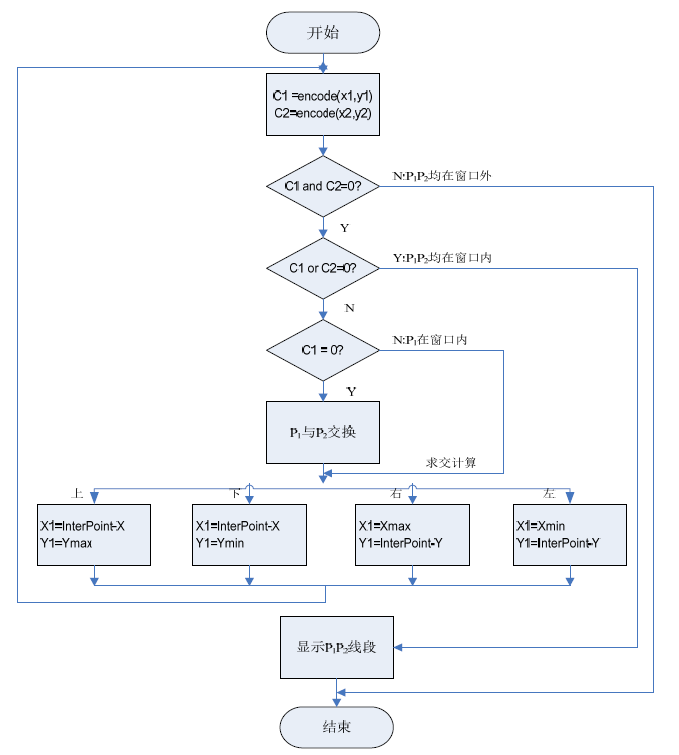
\includegraphics[width=8.55cm,height=9.5cm]{cohen-sutherland-flow.PNG}
    \caption{Cohen-Sutherland算法流程图}
\end{figure}
\begin{figure}[H]
    \centering
    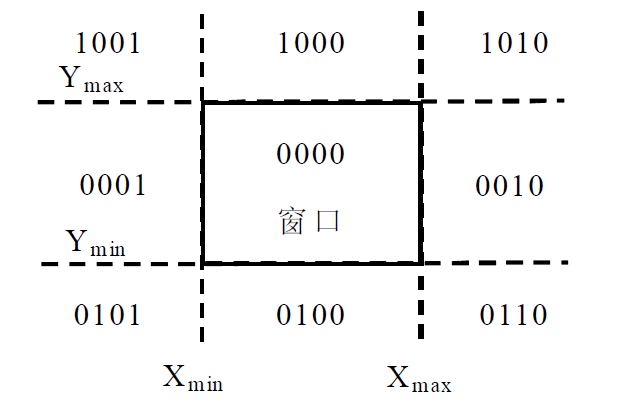
\includegraphics[width=6.28cm,height=4.14cm]{cohen-sutherland-encode.PNG}
    \caption{区域编码}
\end{figure}


\textbf{Liang-Barsky算法}

定义如下8个参数:

\begin{equation*}
    \begin{cases}
        p_1=-\Delta x,q_1=x_0-x_{min}\\
        p_2=\Delta x,q_2=x_{max}-x_0\\
        p_3=-\Delta y,q_3=y_0-y_{min}\\
        p_4=\Delta y,q_4=y_{max}-y_0
    \end{cases}
\end{equation*}

初始化$u_1=0$,$u_2=1$。
对任一组$p_k$和$q_k$,做如下检测:

$p_k=0$时,若$q_k<0$,线段在裁剪窗口外,舍弃该线段,算法结束;

$p_k<0$时,令$u_1$为其本身和$\frac{q_k}{p_k}$中的较大值;

$p_k>0$时,令$u_2$为其本身和$\frac{q_k}{p_k}$中的较小值。

参数更新后,若$u_1>u_2$,舍弃该线段,算法结束。


        
\subsection{对比分析}
\subsubsection{绘制线段}
Naive算法以单位间隔对$x$取样,并根据直线方程计算出相应的$y$坐标,以此得到线段上所有的点。
这一过程需要做大量乘法运算,算法运行速度慢,且对硬件要求较高。
此外,Naive算法不对斜率绝对值大于1和小于1的两种情况区别处理,而是统一地以单位间隔对$x$取样。
因而,当斜率绝对值大于1时,易出现直线取样点稀疏的问题。

DDA算法针对上述缺陷做出了优化,它利用光栅特性消除了直线方程中的乘法,在$x$和$y$方向使用合适的增量逐步推导出各像素点的位置,两种算法的对比如图3所示。
然而,DDA算法仍有不足之处,算法中的浮点运算和取整操作十分耗时,且取整误差的积累会导致长线段的像素位置偏离实际位置。

Bresenham算法在每个已确定的像素点处计算决策参数,选择距离实际线段较近的点作为下一个绘制的点。
相较于DDA算法,这一做法有利于控制绘制出的直线对实际线段的偏离程度。

\begin{figure}[H]
    \centering
    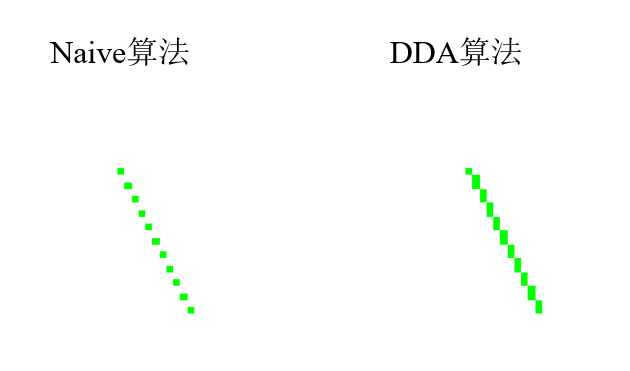
\includegraphics[scale=0.6]{naive-vs-dda.PNG}
    \caption{Naive算法和DDA算法效果对比}
\end{figure}

\subsubsection{绘制曲线}
绘制曲线使用了Bezier曲线和B-Spline曲线,两者在基函数和局部控制能力上存在较大差异。

在基函数方面,Bezier曲线基函数的次数始终等于控制顶点数减1,灵活性不足。
而B-Spline曲线基函数的次数则与控制顶点数无关。

在局部控制能力上,修改Bezier曲线的某一个控制顶点,会影响整条曲线的走向,Bezier曲线在局部性上有所欠缺。
而修改B-Spline曲线的某一个控制顶点,只影响曲线的某一部分,B-Spline曲线的局部性较好。



\section{系统介绍}
% 已完成或拟采用的系统框架、交互逻辑、设计思路等
\subsection{交互逻辑}
目前,系统沿用demo的框架,即命令行和可视化界面两种运行方式。

以命令行方式运行时,
系统逐行读取指令文件,解析指令
并调用cg\underline{ }algorithms.py模块中的相关算法。

以可视化界面运行时,通过鼠标事件获取所需参数,
调用cg\underline{ }algorithms.py模块中的相关算法,
再以可视化方式直接呈现结果。

下面简要介绍可视化界面各个功能的底层实现逻辑和交互方式。

\textbf{设置画笔}

实现逻辑:调用现成的QColorDialog.getColor函数,显示出常见的调色界面,并记录下函数返回值,作为系统当前的画笔颜色。
为MyItem类添加成员变量color,以记录图元颜色。新建MyItem实例时,令该图元的颜色为系统当前的画笔颜色,即可实现要求的功能。

交互方式:点击“文件-设置画笔”,在弹出的颜色选择面板(如图4所示)中选择画笔颜色,选择完毕后点击“OK”按钮。
\begin{figure}[H]
    \centering
    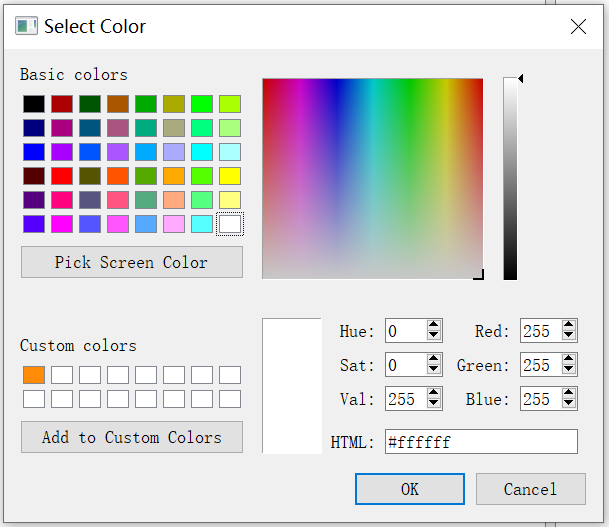
\includegraphics[scale=0.75]{select-color.PNG}
    \caption{颜色选择面板}
\end{figure}

\textbf{重置画布}

实现逻辑:利用现成的QDialog类生成输入窗口,得到输入的数据后,
首先清除item及其在图元列表中的表现,然后根据获得的数据重新设置scene和canvas的宽度和高度。

交互方式:点击“文件-重置画布”,在弹出的输入窗口(如图5所示)中输入画布的宽度和高度值,填写完毕后点击“确定”按钮。
\begin{figure}[H]
    \centering
    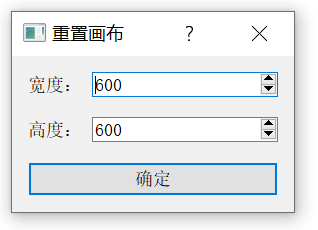
\includegraphics[scale=1]{reset-canvas.PNG}
    \caption{输入窗口}
\end{figure}

\textbf{保存画布}

实现逻辑:调用现成的QFileDialog.getSaveFileName函数,显示出常见的文件保存界面。
再调用QGraphicsView.grab函数截取画布,并将返回的数据保存为位图。

交互方式:点击“文件-保存画布”,在弹出的文件保存窗口(如图6所示)中确定文件名称和保存的位置,完成后点击“保存”按钮。
\begin{figure}[H]
    \centering
    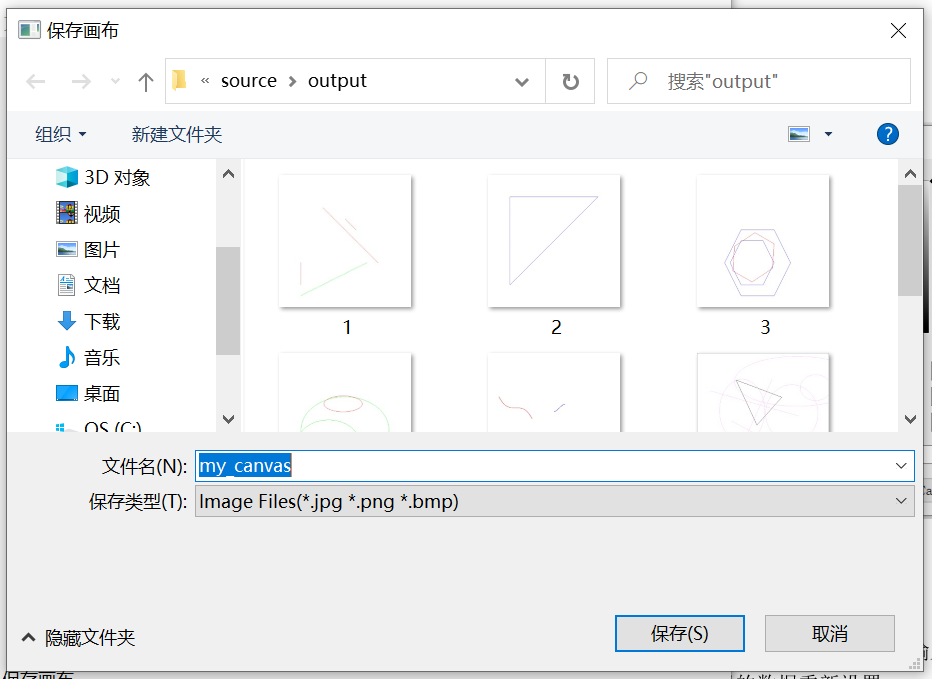
\includegraphics[scale=0.6]{save-canvas.PNG}
    \caption{文件保存窗口}
\end{figure}

\textbf{绘制线段}

实现逻辑:点击鼠标时,将当前坐标作为线段的两个端点,再将两个端点的坐标作为参数传给alg.draw\underline{ }line函数,得到新的线段。
鼠标移动时,将线段第二个端点更新为当前坐标。

交互方式:点击“绘制-线段-算法”,按住鼠标拖拽出线段后松开鼠标,绘制示例如图7所示。
\begin{figure}[H]
    \centering
    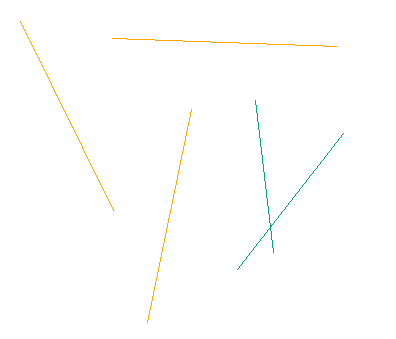
\includegraphics[scale=0.75]{draw-line.PNG}
    \caption{绘制线段示例}
\end{figure}


\textbf{绘制多边形}

实现逻辑:点击鼠标时,如果当前的点在第一个顶点为圆心的半径10个像素的圆内,则认为已经绘制完毕;否则,把当前坐标加入多边形的顶点列表。
鼠标移动时,将顶点列表的最后一个坐标更新为当前坐标。

交互方式:点击“绘制-多边形-算法”,依次点击多边形各个顶点(也可拖拽),最后需再次点击第一个顶点,表示绘制结束,绘制示例如图8所示。
\begin{figure}[H]
    \centering
    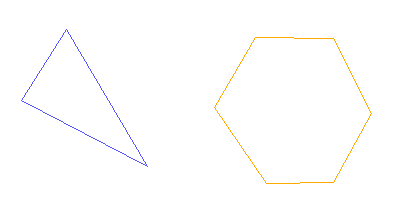
\includegraphics[scale=0.8]{draw-polygen.PNG}
    \caption{绘制多边形示例}
\end{figure}

\textbf{绘制椭圆}

实现逻辑:点击鼠标时,将当前坐标作为椭圆绑定矩形的对角顶点坐标,再将两个顶点的坐标作为参数传给alg.draw\underline{ }ellipse函数,得到新的椭圆。
鼠标移动时,将第二个对角顶点坐标更新为当前坐标。

交互方式:点击“绘制-椭圆”,按住鼠标拖拽出椭圆后松开鼠标,绘制示例如图9所示。
\begin{figure}[H]
    \centering
    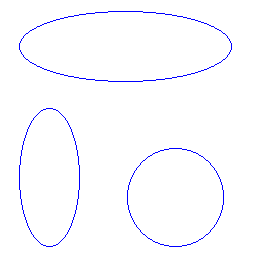
\includegraphics[scale=0.8]{draw-ellipse.PNG}
    \caption{绘制椭圆示例}
\end{figure}

\textbf{绘制曲线}

实现逻辑:点击鼠标时,把当前坐标加入曲线的控制点列表。鼠标移动时,将控制点列表的最后一个坐标更新为当前坐标。按回车键时,绘制结束。

交互方式:点击“绘制-曲线-算法”,依次点击曲线各个控制点,最后按回车键表示绘制结束,绘制示例如图10所示。
\begin{figure}[H]
    \centering
    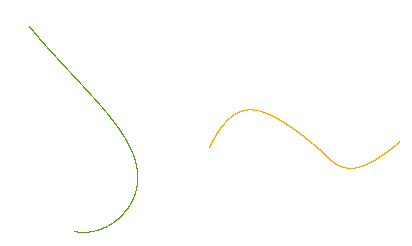
\includegraphics[scale=0.8]{draw-curve.PNG}
    \caption{绘制曲线示例}
\end{figure}

\textbf{平移}

实现逻辑:点击鼠标时,将当前坐标作为平移向量的起点和终点坐标,再将平移向量的坐标作为参数传给alg.translate函数,得到平移后的图元。
鼠标移动时,将平移向量的终点坐标更新为当前坐标。

交互方式:点击“编辑-平移”,按住鼠标将图元拖拽到目标位置,再松开鼠标,示例如图11所示。
\begin{figure}[H]
    \centering
    \subfigure[平移前]{
    \begin{minipage}{7cm}
        \centering
        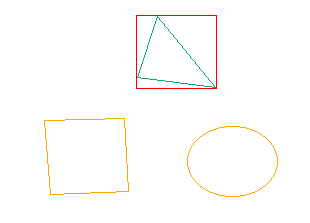
\includegraphics[scale=0.8]{before-translate.PNG}
    \end{minipage}}
    \subfigure[平移后]{
        \begin{minipage}{7cm}
            \centering
            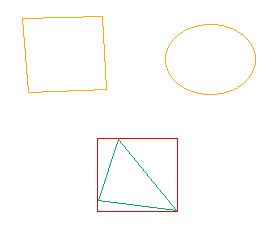
\includegraphics[scale=0.8]{after-translate.PNG}
        \end{minipage}}
        \caption{平移示例}
        %\label{fig:1}
\end{figure}

\textbf{旋转}

实现逻辑:旋转分为两个阶段,第一阶段,点击鼠标时将当前坐标作为旋转中心,移动鼠标时将旋转中心更新为当前坐标;
第二阶段,点击鼠标时将当前坐标作为旋转弧线的起点和终点,移动鼠标时将弧线的终点更新为当前坐标。
再将旋转中心坐标和根据弧线计算出的旋转角度作为参数传给alg.rotate函数,得到旋转后的图元。

交互方式:点击“编辑-旋转”,首先点击旋转中心,接着按住鼠标拖拽出旋转的弧线,再松开鼠标,示例如图12所示。
\begin{figure}[H]
    \centering
    \subfigure[旋转前]{
    \begin{minipage}{7cm}
        \centering
        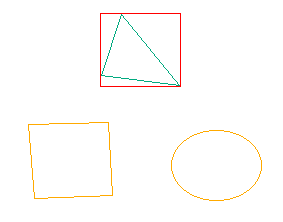
\includegraphics[scale=0.8]{before-rotate.PNG}
    \end{minipage}}
    \subfigure[旋转后]{
        \begin{minipage}{7cm}
            \centering
            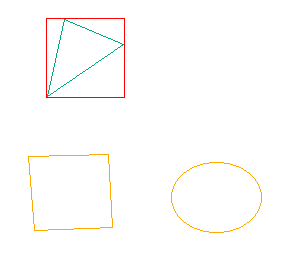
\includegraphics[scale=0.8]{after-rotate.PNG}
        \end{minipage}}
        \caption{旋转示例}
        %\label{fig:1}
\end{figure}

\textbf{缩放}

实现逻辑:缩放分为两个阶段,第一阶段,点击鼠标时将当前坐标作为缩放中心,移动鼠标时将缩放中心更新为当前坐标;
第二阶段,点击鼠标时将当前坐标作为缩放线段的起点和终点,移动鼠标时将缩放线段的终点更新为当前坐标。
令缩放倍数等于缩放线段长度与80的比值,将缩放中心坐标和缩放倍数作为参数传给alg.scale函数,得到缩放后的图元。

交互方式:点击“编辑-缩放”,首先点击缩放中心,接着按住鼠标拖拽指导图元变为目标大小,再松开鼠标,示例如图13所示。
\begin{figure}[H]
    \centering
    \subfigure[缩放前]{
    \begin{minipage}{7cm}
        \centering
        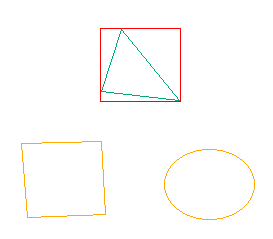
\includegraphics[scale=0.8]{before-scale.PNG}
    \end{minipage}}
    \subfigure[缩放后]{
        \begin{minipage}{7cm}
            \centering
            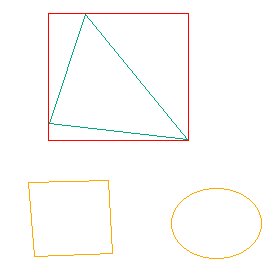
\includegraphics[scale=0.8]{after-scale.PNG}
        \end{minipage}}
        \caption{缩放示例}
        %\label{fig:1}
\end{figure}

\textbf{裁剪}

实现逻辑:点击鼠标时,将当前坐标作为裁剪窗口的对角顶点坐标,再将两个顶点坐标作为参数传给alg.clip函数,得到裁剪后的图元。
鼠标移动时,将裁剪窗口的第二个对角顶点坐标更新为当前坐标。

交互方式:点击“编辑-裁剪”,按住鼠标拖拽出裁剪矩形的对角线,得到裁剪后的线段,示例如图14所示。
\begin{figure}[H]
    \centering
    \subfigure[裁剪前]{
    \begin{minipage}{7cm}
        \centering
        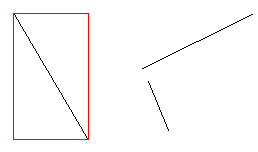
\includegraphics[scale=0.8]{before-clip.PNG}
    \end{minipage}}
    \subfigure[裁剪后]{
        \begin{minipage}{7cm}
            \centering
            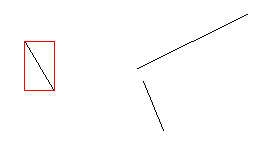
\includegraphics[scale=0.8]{after-clip.PNG}
        \end{minipage}}
        \caption{裁剪示例}
        %\label{fig:1}
\end{figure}



\subsection{设计思路}
后续将着重优化图形界面,计划在图形界面中做出以下修改:

(1)对用户隐藏图元序号,可以直接通过鼠标选中图元,并对图元进行平移操作;

(2)优化曲线绘制交互,用鼠标操作代替按下回车键来标志绘制结束;

(3)优化平移功能,目前在画布任意处拖拽出平移向量都能平移图元,
但这一操作与常见画图软件的平移操作不一致。
后续,考虑将平移向量的起点限定在选定图元的绑定矩形中。

(4)优化裁剪功能,目前裁剪时随着裁剪窗口的变化,裁剪后的线段实时更新,
不便观察完整线段与裁剪窗口的位置关系。
后续,考虑在裁剪窗口未确定时保留原来的完整线段,使操作更为自然便利。

(5)目前保存画布时调用grab函数,然而当启用滚动条时,这一方法无法保存完整的画布。
因此,11月提交的代码中禁用滚动条,以保存完整画布。
后续,考虑启用滚动条,以便扩大画布尺寸。

(6)优化图形界面,目前绘制图元、编辑图元都需要点击菜单栏若干次,操作不够便捷。
后续,考虑将各个功能分散为菜单栏的图标。

(7)添加额外的功能,如多边形填充、撤销、复制等。


\section{总结}
11月提交中,运用了目前已讲到图形学基础知识,并自学了解了绘制图元和编辑图元的若干算法。
通过实现所有指令的算法和图形界面,加深了对图形显示原理的理解。
同时,通过反复测试找出了之前提交代码中的若干错误,如公式错误、代码编写错误等。
在纠正代码错误的过程中,加深了对算法公式推导过程和Python语言的理解程度。

目前对图形界面的理解较浅,尚未基于demo的图形界面框架做出显著改动,
主要着眼于在图形界面实现实验要求的基本功能。
后续将着重优化图形界面,使得整个图形学系统功能更为多样,使用更为便利。
\\\\\\



\bibliographystyle{plain}
\begin{thebibliography}{99}
% 注明在实现作业过程中使用的参考资料,包括技术博客等
\bibitem{ref1} 孙正兴等. 计算机图形学教程[M]. 机械工业出版社, 2006.
\bibitem{ref2} Qt 5.15手册\\\url{https://doc.qt.io/qt-5/index.html}
\bibitem{ref3} 计算向量夹角\\\url{https://blog.csdn.net/qq_42423940/article/details/83757427}
\bibitem{ref4} QListWidget右键菜单\\\url{https://blog.csdn.net/qq_42365249/article/details/106651354}
\bibitem{ref5} PyQt 5菜单栏、工具栏和状态栏使用\\\url{https://www.cnblogs.com/ygzhaof/p/10070523.html}
\bibitem{ref6} QToolButtton简介\\\url{https://blog.csdn.net/qq_17351161/article/details/102917153}
\bibitem{ref7} 多边形填充算法\\\url{https://blog.csdn.net/keneyr/article/details/83747501}
\bibitem{ref8} 多边形裁剪Weiler-Atherton算法\\\url{https://blog.csdn.net/yangxi_pekin/article/details/37738219} 
\end{thebibliography}

\end{document}